There are different types of DC-DC converters used for PV module integration. However, the main topologies of power converters used in MICs are buck, boost and non-inverting buck-boost DC-DC converters. The functionality and the advantages and disadvantages of these three topologies will be analyzed in this section.

\subsection{Buck converter\label{Buck-C}}

A buck converter is one of the simplest DC-DC converters with the task of decreasing the input voltage. The required components are a DC source for the input voltage, two switches (a diode and a transistor), an inductor, a capacitor and a load. The equivalent diagram in figure \ref{Buck-converter} illustrates a buck converter. 

A buck converter performs in two operating states. 
During the first state, the MOSFET is conducting and the diode is reversed bias thus working as an open-circuit. The voltage drop  then is divided between the inductor and the load. Since the voltage is split, the voltage drop on the load is lower than the input voltage. In addition, both the capacitor and the inductor are being charged. In the second state, the MOSFET is switched off and the current flows through the diode as it is forward-biased. During this state, the inductor works as a current source and the capacitor stabilizes the voltage \cite{schematicbuckandboost}.

\begin{figure}[H]
	\begin{center}
		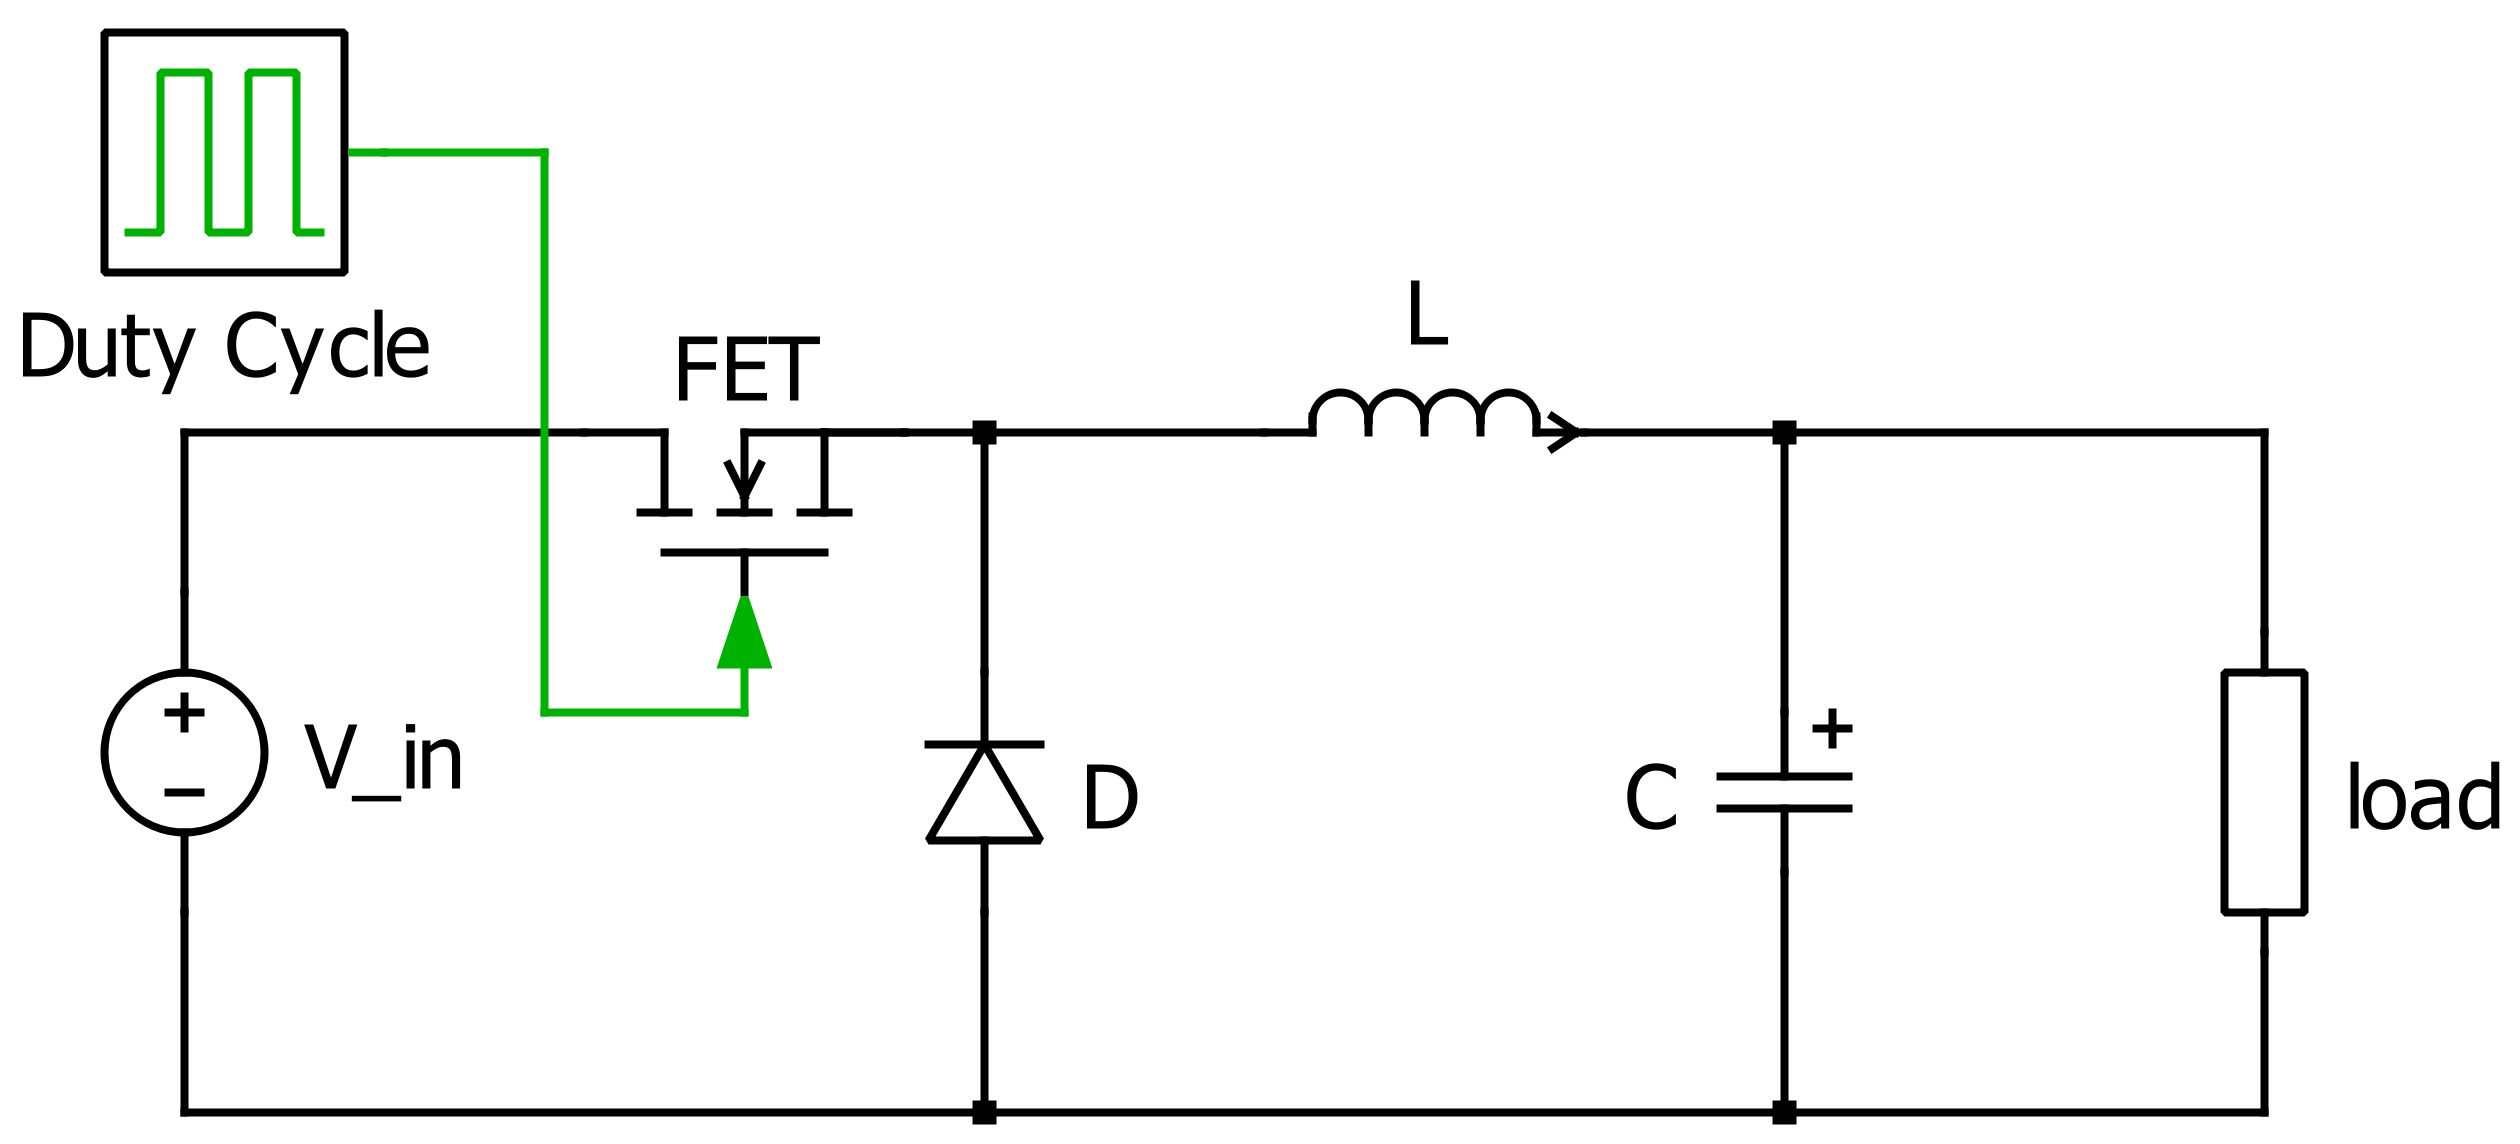
\includegraphics[width=0.7\textwidth]{../Pictures/Buck-converter}
		\caption{Equivalent circuit for the DC-DC buck converter.}
		\label{Buck-converter}
	\end{center}	
\end{figure}

The main advantage of using a buck converter is that the structure is very simple and only one controlled  switch is needed. Also, the component count and thus cost of implementation is low. Furthermore, the buck converter can reach efficiencies up to 99\% \cite{Efficiencybuck}. However, this topology is not very versatile since it does not allow the increase of output voltage with respect to the input.

\subsection{Boost converter\label{Boost-C}}

A boost converter is another type of DC-DC converter similar to the buck converter but instead of lowering the output voltage, it produces a higher electrical potential at the output with respect to that at the input. 
The circuit consists of two switches (a transistor and a diode), an inductor, a capacitor, a load and a DC source for the input voltage. Figure \ref{Boost-converter} shows the equivalent circuit diagram for the boost converter with the aforementioned components. %%\cite{Reddy2011}

\begin{figure}[H]
	\begin{center}
		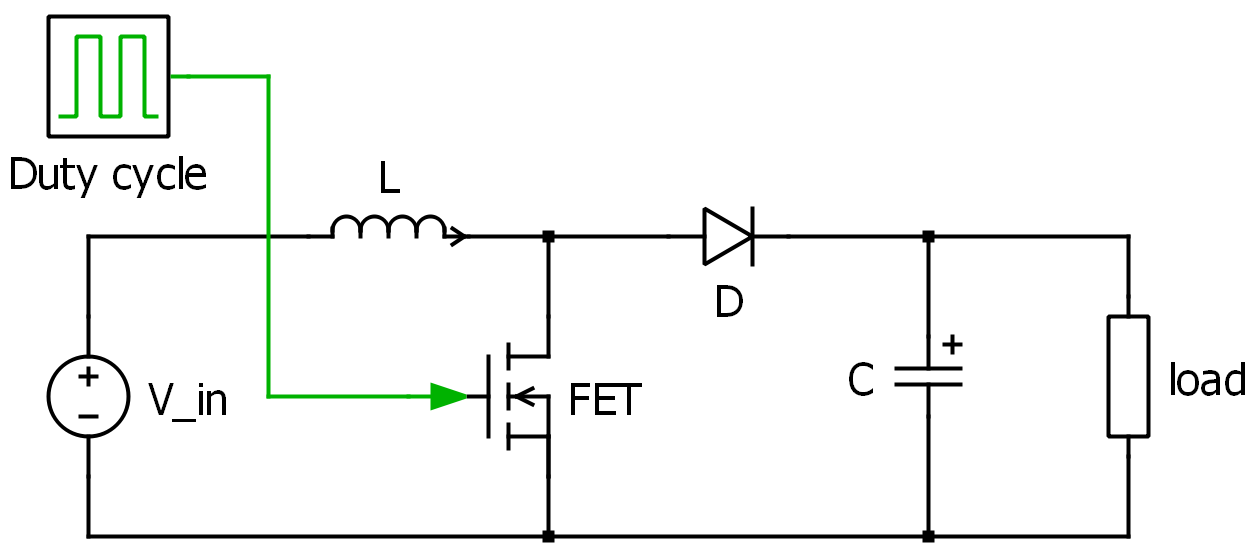
\includegraphics[width=0.75\textwidth]{../Pictures/Boost-converter}
		\caption{Equivalent circuit for the DC-DC boost converter.}
		\label{Boost-converter}
	\end{center}	
\end{figure}

\vspace{1cm}
Similarly to the buck converter, this topology has two states. When the MOSFET is on, the current flows only trough the inductor because the diode  is reverse biased. Energy is then stored in the inductor, which voltage is equal to the input voltage, and current increases. Meanwhile, the capacitor releases the previously stored energy to the load.
During the second state, when the MOSFET is turned off, the current loops trough the inductor, diode, capacitor and the load. Since the inductor had been previously charged, it now works as a current source in series with the voltage source of the circuit. The voltage across the load is then risen with respect to that at the input. Furthermore, the capacitor is being charged \cite{schematicbuckandboost}. It is also a cheap converter and it is easy to control \cite{advantagebuckboost}. However, as it happened with the buck, the boost converter is also limited to rising the voltage and lowering it cannot be achieved. The boost converter voltage gain has a non-linear transfer function that can produce cause damage to the system's components if the duty cycle is not properly limited to a maximum values.
 
